% Options for packages loaded elsewhere
\PassOptionsToPackage{unicode}{hyperref}
\PassOptionsToPackage{hyphens}{url}
\PassOptionsToPackage{dvipsnames,svgnames,x11names}{xcolor}
%
\documentclass[
  letterpaper,
  DIV=11,
  numbers=noendperiod]{scrartcl}

\usepackage{amsmath,amssymb}
\usepackage{iftex}
\ifPDFTeX
  \usepackage[T1]{fontenc}
  \usepackage[utf8]{inputenc}
  \usepackage{textcomp} % provide euro and other symbols
\else % if luatex or xetex
  \usepackage{unicode-math}
  \defaultfontfeatures{Scale=MatchLowercase}
  \defaultfontfeatures[\rmfamily]{Ligatures=TeX,Scale=1}
\fi
\usepackage{lmodern}
\ifPDFTeX\else  
    % xetex/luatex font selection
\fi
% Use upquote if available, for straight quotes in verbatim environments
\IfFileExists{upquote.sty}{\usepackage{upquote}}{}
\IfFileExists{microtype.sty}{% use microtype if available
  \usepackage[]{microtype}
  \UseMicrotypeSet[protrusion]{basicmath} % disable protrusion for tt fonts
}{}
\makeatletter
\@ifundefined{KOMAClassName}{% if non-KOMA class
  \IfFileExists{parskip.sty}{%
    \usepackage{parskip}
  }{% else
    \setlength{\parindent}{0pt}
    \setlength{\parskip}{6pt plus 2pt minus 1pt}}
}{% if KOMA class
  \KOMAoptions{parskip=half}}
\makeatother
\usepackage{xcolor}
\setlength{\emergencystretch}{3em} % prevent overfull lines
\setcounter{secnumdepth}{-\maxdimen} % remove section numbering
% Make \paragraph and \subparagraph free-standing
\makeatletter
\ifx\paragraph\undefined\else
  \let\oldparagraph\paragraph
  \renewcommand{\paragraph}{
    \@ifstar
      \xxxParagraphStar
      \xxxParagraphNoStar
  }
  \newcommand{\xxxParagraphStar}[1]{\oldparagraph*{#1}\mbox{}}
  \newcommand{\xxxParagraphNoStar}[1]{\oldparagraph{#1}\mbox{}}
\fi
\ifx\subparagraph\undefined\else
  \let\oldsubparagraph\subparagraph
  \renewcommand{\subparagraph}{
    \@ifstar
      \xxxSubParagraphStar
      \xxxSubParagraphNoStar
  }
  \newcommand{\xxxSubParagraphStar}[1]{\oldsubparagraph*{#1}\mbox{}}
  \newcommand{\xxxSubParagraphNoStar}[1]{\oldsubparagraph{#1}\mbox{}}
\fi
\makeatother

\usepackage{color}
\usepackage{fancyvrb}
\newcommand{\VerbBar}{|}
\newcommand{\VERB}{\Verb[commandchars=\\\{\}]}
\DefineVerbatimEnvironment{Highlighting}{Verbatim}{commandchars=\\\{\}}
% Add ',fontsize=\small' for more characters per line
\usepackage{framed}
\definecolor{shadecolor}{RGB}{241,243,245}
\newenvironment{Shaded}{\begin{snugshade}}{\end{snugshade}}
\newcommand{\AlertTok}[1]{\textcolor[rgb]{0.68,0.00,0.00}{#1}}
\newcommand{\AnnotationTok}[1]{\textcolor[rgb]{0.37,0.37,0.37}{#1}}
\newcommand{\AttributeTok}[1]{\textcolor[rgb]{0.40,0.45,0.13}{#1}}
\newcommand{\BaseNTok}[1]{\textcolor[rgb]{0.68,0.00,0.00}{#1}}
\newcommand{\BuiltInTok}[1]{\textcolor[rgb]{0.00,0.23,0.31}{#1}}
\newcommand{\CharTok}[1]{\textcolor[rgb]{0.13,0.47,0.30}{#1}}
\newcommand{\CommentTok}[1]{\textcolor[rgb]{0.37,0.37,0.37}{#1}}
\newcommand{\CommentVarTok}[1]{\textcolor[rgb]{0.37,0.37,0.37}{\textit{#1}}}
\newcommand{\ConstantTok}[1]{\textcolor[rgb]{0.56,0.35,0.01}{#1}}
\newcommand{\ControlFlowTok}[1]{\textcolor[rgb]{0.00,0.23,0.31}{\textbf{#1}}}
\newcommand{\DataTypeTok}[1]{\textcolor[rgb]{0.68,0.00,0.00}{#1}}
\newcommand{\DecValTok}[1]{\textcolor[rgb]{0.68,0.00,0.00}{#1}}
\newcommand{\DocumentationTok}[1]{\textcolor[rgb]{0.37,0.37,0.37}{\textit{#1}}}
\newcommand{\ErrorTok}[1]{\textcolor[rgb]{0.68,0.00,0.00}{#1}}
\newcommand{\ExtensionTok}[1]{\textcolor[rgb]{0.00,0.23,0.31}{#1}}
\newcommand{\FloatTok}[1]{\textcolor[rgb]{0.68,0.00,0.00}{#1}}
\newcommand{\FunctionTok}[1]{\textcolor[rgb]{0.28,0.35,0.67}{#1}}
\newcommand{\ImportTok}[1]{\textcolor[rgb]{0.00,0.46,0.62}{#1}}
\newcommand{\InformationTok}[1]{\textcolor[rgb]{0.37,0.37,0.37}{#1}}
\newcommand{\KeywordTok}[1]{\textcolor[rgb]{0.00,0.23,0.31}{\textbf{#1}}}
\newcommand{\NormalTok}[1]{\textcolor[rgb]{0.00,0.23,0.31}{#1}}
\newcommand{\OperatorTok}[1]{\textcolor[rgb]{0.37,0.37,0.37}{#1}}
\newcommand{\OtherTok}[1]{\textcolor[rgb]{0.00,0.23,0.31}{#1}}
\newcommand{\PreprocessorTok}[1]{\textcolor[rgb]{0.68,0.00,0.00}{#1}}
\newcommand{\RegionMarkerTok}[1]{\textcolor[rgb]{0.00,0.23,0.31}{#1}}
\newcommand{\SpecialCharTok}[1]{\textcolor[rgb]{0.37,0.37,0.37}{#1}}
\newcommand{\SpecialStringTok}[1]{\textcolor[rgb]{0.13,0.47,0.30}{#1}}
\newcommand{\StringTok}[1]{\textcolor[rgb]{0.13,0.47,0.30}{#1}}
\newcommand{\VariableTok}[1]{\textcolor[rgb]{0.07,0.07,0.07}{#1}}
\newcommand{\VerbatimStringTok}[1]{\textcolor[rgb]{0.13,0.47,0.30}{#1}}
\newcommand{\WarningTok}[1]{\textcolor[rgb]{0.37,0.37,0.37}{\textit{#1}}}

\providecommand{\tightlist}{%
  \setlength{\itemsep}{0pt}\setlength{\parskip}{0pt}}\usepackage{longtable,booktabs,array}
\usepackage{calc} % for calculating minipage widths
% Correct order of tables after \paragraph or \subparagraph
\usepackage{etoolbox}
\makeatletter
\patchcmd\longtable{\par}{\if@noskipsec\mbox{}\fi\par}{}{}
\makeatother
% Allow footnotes in longtable head/foot
\IfFileExists{footnotehyper.sty}{\usepackage{footnotehyper}}{\usepackage{footnote}}
\makesavenoteenv{longtable}
\usepackage{graphicx}
\makeatletter
\def\maxwidth{\ifdim\Gin@nat@width>\linewidth\linewidth\else\Gin@nat@width\fi}
\def\maxheight{\ifdim\Gin@nat@height>\textheight\textheight\else\Gin@nat@height\fi}
\makeatother
% Scale images if necessary, so that they will not overflow the page
% margins by default, and it is still possible to overwrite the defaults
% using explicit options in \includegraphics[width, height, ...]{}
\setkeys{Gin}{width=\maxwidth,height=\maxheight,keepaspectratio}
% Set default figure placement to htbp
\makeatletter
\def\fps@figure{htbp}
\makeatother

\KOMAoption{captions}{tableheading}
\makeatletter
\@ifpackageloaded{caption}{}{\usepackage{caption}}
\AtBeginDocument{%
\ifdefined\contentsname
  \renewcommand*\contentsname{Table of contents}
\else
  \newcommand\contentsname{Table of contents}
\fi
\ifdefined\listfigurename
  \renewcommand*\listfigurename{List of Figures}
\else
  \newcommand\listfigurename{List of Figures}
\fi
\ifdefined\listtablename
  \renewcommand*\listtablename{List of Tables}
\else
  \newcommand\listtablename{List of Tables}
\fi
\ifdefined\figurename
  \renewcommand*\figurename{Figure}
\else
  \newcommand\figurename{Figure}
\fi
\ifdefined\tablename
  \renewcommand*\tablename{Table}
\else
  \newcommand\tablename{Table}
\fi
}
\@ifpackageloaded{float}{}{\usepackage{float}}
\floatstyle{ruled}
\@ifundefined{c@chapter}{\newfloat{codelisting}{h}{lop}}{\newfloat{codelisting}{h}{lop}[chapter]}
\floatname{codelisting}{Listing}
\newcommand*\listoflistings{\listof{codelisting}{List of Listings}}
\makeatother
\makeatletter
\makeatother
\makeatletter
\@ifpackageloaded{caption}{}{\usepackage{caption}}
\@ifpackageloaded{subcaption}{}{\usepackage{subcaption}}
\makeatother

\ifLuaTeX
  \usepackage{selnolig}  % disable illegal ligatures
\fi
\usepackage{bookmark}

\IfFileExists{xurl.sty}{\usepackage{xurl}}{} % add URL line breaks if available
\urlstyle{same} % disable monospaced font for URLs
\hypersetup{
  pdftitle={Class13:Transcriptomics},
  pdfauthor={Isabel Philip (A16855684)},
  colorlinks=true,
  linkcolor={blue},
  filecolor={Maroon},
  citecolor={Blue},
  urlcolor={Blue},
  pdfcreator={LaTeX via pandoc}}


\title{Class13:Transcriptomics}
\author{Isabel Philip (A16855684)}
\date{}

\begin{document}
\maketitle


Today we will analyze the data from a published RNA-seq experiment where
airway smooth muscle cells were treated with dexamethasone, a synthetic
glucocorticoid steroid with anti-inflammatory effects (Himes et
al.~2014).

\begin{Shaded}
\begin{Highlighting}[]
\FunctionTok{library}\NormalTok{(BiocManager)}
\FunctionTok{library}\NormalTok{(DESeq2)}
\end{Highlighting}
\end{Shaded}

\begin{verbatim}
Loading required package: S4Vectors
\end{verbatim}

\begin{verbatim}
Loading required package: stats4
\end{verbatim}

\begin{verbatim}
Loading required package: BiocGenerics
\end{verbatim}

\begin{verbatim}

Attaching package: 'BiocGenerics'
\end{verbatim}

\begin{verbatim}
The following objects are masked from 'package:stats':

    IQR, mad, sd, var, xtabs
\end{verbatim}

\begin{verbatim}
The following objects are masked from 'package:base':

    anyDuplicated, aperm, append, as.data.frame, basename, cbind,
    colnames, dirname, do.call, duplicated, eval, evalq, Filter, Find,
    get, grep, grepl, intersect, is.unsorted, lapply, Map, mapply,
    match, mget, order, paste, pmax, pmax.int, pmin, pmin.int,
    Position, rank, rbind, Reduce, rownames, sapply, saveRDS, setdiff,
    table, tapply, union, unique, unsplit, which.max, which.min
\end{verbatim}

\begin{verbatim}

Attaching package: 'S4Vectors'
\end{verbatim}

\begin{verbatim}
The following object is masked from 'package:utils':

    findMatches
\end{verbatim}

\begin{verbatim}
The following objects are masked from 'package:base':

    expand.grid, I, unname
\end{verbatim}

\begin{verbatim}
Loading required package: IRanges
\end{verbatim}

\begin{verbatim}
Loading required package: GenomicRanges
\end{verbatim}

\begin{verbatim}
Loading required package: GenomeInfoDb
\end{verbatim}

\begin{verbatim}
Loading required package: SummarizedExperiment
\end{verbatim}

\begin{verbatim}
Loading required package: MatrixGenerics
\end{verbatim}

\begin{verbatim}
Loading required package: matrixStats
\end{verbatim}

\begin{verbatim}

Attaching package: 'MatrixGenerics'
\end{verbatim}

\begin{verbatim}
The following objects are masked from 'package:matrixStats':

    colAlls, colAnyNAs, colAnys, colAvgsPerRowSet, colCollapse,
    colCounts, colCummaxs, colCummins, colCumprods, colCumsums,
    colDiffs, colIQRDiffs, colIQRs, colLogSumExps, colMadDiffs,
    colMads, colMaxs, colMeans2, colMedians, colMins, colOrderStats,
    colProds, colQuantiles, colRanges, colRanks, colSdDiffs, colSds,
    colSums2, colTabulates, colVarDiffs, colVars, colWeightedMads,
    colWeightedMeans, colWeightedMedians, colWeightedSds,
    colWeightedVars, rowAlls, rowAnyNAs, rowAnys, rowAvgsPerColSet,
    rowCollapse, rowCounts, rowCummaxs, rowCummins, rowCumprods,
    rowCumsums, rowDiffs, rowIQRDiffs, rowIQRs, rowLogSumExps,
    rowMadDiffs, rowMads, rowMaxs, rowMeans2, rowMedians, rowMins,
    rowOrderStats, rowProds, rowQuantiles, rowRanges, rowRanks,
    rowSdDiffs, rowSds, rowSums2, rowTabulates, rowVarDiffs, rowVars,
    rowWeightedMads, rowWeightedMeans, rowWeightedMedians,
    rowWeightedSds, rowWeightedVars
\end{verbatim}

\begin{verbatim}
Loading required package: Biobase
\end{verbatim}

\begin{verbatim}
Welcome to Bioconductor

    Vignettes contain introductory material; view with
    'browseVignettes()'. To cite Bioconductor, see
    'citation("Biobase")', and for packages 'citation("pkgname")'.
\end{verbatim}

\begin{verbatim}

Attaching package: 'Biobase'
\end{verbatim}

\begin{verbatim}
The following object is masked from 'package:MatrixGenerics':

    rowMedians
\end{verbatim}

\begin{verbatim}
The following objects are masked from 'package:matrixStats':

    anyMissing, rowMedians
\end{verbatim}

\section{1. Import countData and
colData}\label{import-countdata-and-coldata}

There are 2 datasets I need to import/ read/ - \texttt{countData} the
transcript counts per gene (rows) in the different experiements. -
\texttt{colData} infomration about the columns (i.e.~experiments) in
\texttt{countData}.

\begin{Shaded}
\begin{Highlighting}[]
\NormalTok{counts }\OtherTok{\textless{}{-}} \FunctionTok{read.csv}\NormalTok{(}\StringTok{"airway\_scaledcounts.csv"}\NormalTok{, }\AttributeTok{row.names=}\DecValTok{1}\NormalTok{)}
\NormalTok{metadata }\OtherTok{\textless{}{-}} \FunctionTok{read.csv}\NormalTok{(}\StringTok{"airway\_metadata.csv"}\NormalTok{)}
\end{Highlighting}
\end{Shaded}

Can have a sneak peak with \texttt{head()}

\begin{Shaded}
\begin{Highlighting}[]
\FunctionTok{head}\NormalTok{(counts)}
\end{Highlighting}
\end{Shaded}

\begin{verbatim}
                SRR1039508 SRR1039509 SRR1039512 SRR1039513 SRR1039516
ENSG00000000003        723        486        904        445       1170
ENSG00000000005          0          0          0          0          0
ENSG00000000419        467        523        616        371        582
ENSG00000000457        347        258        364        237        318
ENSG00000000460         96         81         73         66        118
ENSG00000000938          0          0          1          0          2
                SRR1039517 SRR1039520 SRR1039521
ENSG00000000003       1097        806        604
ENSG00000000005          0          0          0
ENSG00000000419        781        417        509
ENSG00000000457        447        330        324
ENSG00000000460         94        102         74
ENSG00000000938          0          0          0
\end{verbatim}

\begin{Shaded}
\begin{Highlighting}[]
\FunctionTok{head}\NormalTok{(metadata)}
\end{Highlighting}
\end{Shaded}

\begin{verbatim}
          id     dex celltype     geo_id
1 SRR1039508 control   N61311 GSM1275862
2 SRR1039509 treated   N61311 GSM1275863
3 SRR1039512 control  N052611 GSM1275866
4 SRR1039513 treated  N052611 GSM1275867
5 SRR1039516 control  N080611 GSM1275870
6 SRR1039517 treated  N080611 GSM1275871
\end{verbatim}

\begin{quote}
Q1. How many genes are in this dataset?
\end{quote}

There are 38694 genes in this data set.

\begin{Shaded}
\begin{Highlighting}[]
\FunctionTok{nrow}\NormalTok{(counts)}
\end{Highlighting}
\end{Shaded}

\begin{verbatim}
[1] 38694
\end{verbatim}

\begin{quote}
Q2. How many `control' cell lines do we have?
\end{quote}

There are 4 ``control'' cell lines.

\begin{Shaded}
\begin{Highlighting}[]
\FunctionTok{sum}\NormalTok{(metadata}\SpecialCharTok{$}\NormalTok{dex }\SpecialCharTok{==}\StringTok{"control"}\NormalTok{)}
\end{Highlighting}
\end{Shaded}

\begin{verbatim}
[1] 4
\end{verbatim}

\section{2. Toy differential gene
expression}\label{toy-differential-gene-expression}

\begin{Shaded}
\begin{Highlighting}[]
\NormalTok{control }\OtherTok{\textless{}{-}}\NormalTok{ metadata[metadata[,}\StringTok{"dex"}\NormalTok{]}\SpecialCharTok{==}\StringTok{"control"}\NormalTok{,]}
\NormalTok{control.counts }\OtherTok{\textless{}{-}}\NormalTok{ counts[ ,control}\SpecialCharTok{$}\NormalTok{id]}
\NormalTok{control.mean }\OtherTok{\textless{}{-}} \FunctionTok{rowSums}\NormalTok{( control.counts )}\SpecialCharTok{/}\DecValTok{4} 
\CommentTok{\#head(control.mean)}
\end{Highlighting}
\end{Shaded}

OR

\begin{Shaded}
\begin{Highlighting}[]
\FunctionTok{library}\NormalTok{(dplyr)}
\end{Highlighting}
\end{Shaded}

\begin{verbatim}

Attaching package: 'dplyr'
\end{verbatim}

\begin{verbatim}
The following object is masked from 'package:Biobase':

    combine
\end{verbatim}

\begin{verbatim}
The following object is masked from 'package:matrixStats':

    count
\end{verbatim}

\begin{verbatim}
The following objects are masked from 'package:GenomicRanges':

    intersect, setdiff, union
\end{verbatim}

\begin{verbatim}
The following object is masked from 'package:GenomeInfoDb':

    intersect
\end{verbatim}

\begin{verbatim}
The following objects are masked from 'package:IRanges':

    collapse, desc, intersect, setdiff, slice, union
\end{verbatim}

\begin{verbatim}
The following objects are masked from 'package:S4Vectors':

    first, intersect, rename, setdiff, setequal, union
\end{verbatim}

\begin{verbatim}
The following objects are masked from 'package:BiocGenerics':

    combine, intersect, setdiff, union
\end{verbatim}

\begin{verbatim}
The following objects are masked from 'package:stats':

    filter, lag
\end{verbatim}

\begin{verbatim}
The following objects are masked from 'package:base':

    intersect, setdiff, setequal, union
\end{verbatim}

\begin{Shaded}
\begin{Highlighting}[]
\NormalTok{control }\OtherTok{\textless{}{-}}\NormalTok{ metadata }\SpecialCharTok{\%\textgreater{}\%} \FunctionTok{filter}\NormalTok{(dex}\SpecialCharTok{==}\StringTok{"control"}\NormalTok{)}
\NormalTok{control.counts }\OtherTok{\textless{}{-}}\NormalTok{ counts }\SpecialCharTok{\%\textgreater{}\%} \FunctionTok{select}\NormalTok{(control}\SpecialCharTok{$}\NormalTok{id) }
\NormalTok{control.mean }\OtherTok{\textless{}{-}} \FunctionTok{rowSums}\NormalTok{(control.counts)}\SpecialCharTok{/}\DecValTok{4}
\CommentTok{\#head(control.mean)}
\end{Highlighting}
\end{Shaded}

\begin{quote}
Q3. How would you make the above code in either approach more robust? Is
there a function that could help here?
\end{quote}

rowSums

We can find the average (mean) count values per gene for all the
``control'' experiments and compare it to the mean values of the
``treated''.

\begin{itemize}
\tightlist
\item
  Extract all ``control'' columns/ experiments from the \texttt{counts}
  data.
\item
  Find the mean value for each gene in these columns
\end{itemize}

\begin{Shaded}
\begin{Highlighting}[]
\NormalTok{control.inds }\OtherTok{\textless{}{-}}\NormalTok{ metadata}\SpecialCharTok{$}\NormalTok{dex }\SpecialCharTok{==} \StringTok{"control"}
\NormalTok{control.count }\OtherTok{\textless{}{-}}\NormalTok{ counts[ ,control.inds]}
\CommentTok{\#will give 4 columns from the original data }
\end{Highlighting}
\end{Shaded}

\begin{Shaded}
\begin{Highlighting}[]
\FunctionTok{dim}\NormalTok{(control.counts)}
\end{Highlighting}
\end{Shaded}

\begin{verbatim}
[1] 38694     4
\end{verbatim}

\begin{quote}
Mean from the summary of the columns (mean across the rows) - making
into one column
\end{quote}

Now find the row wise mean

\begin{Shaded}
\begin{Highlighting}[]
\NormalTok{control.mean }\OtherTok{\textless{}{-}} \FunctionTok{rowSums}\NormalTok{(control.counts)}\SpecialCharTok{/}\DecValTok{4}
\CommentTok{\#dividing by 4 since there are 4 control groups }
\FunctionTok{head}\NormalTok{(control.mean)}
\end{Highlighting}
\end{Shaded}

\begin{verbatim}
ENSG00000000003 ENSG00000000005 ENSG00000000419 ENSG00000000457 ENSG00000000460 
         900.75            0.00          520.50          339.75           97.25 
ENSG00000000938 
           0.75 
\end{verbatim}

\begin{quote}
Q4. Follow the same procedure for the \texttt{treated} samples
(i.e.~calculate the mean per gene across drug treated samples and assign
to a labeled vector called \texttt{treated.mean})
\end{quote}

\begin{Shaded}
\begin{Highlighting}[]
\FunctionTok{library}\NormalTok{(dplyr)}
\NormalTok{treat }\OtherTok{\textless{}{-}}\NormalTok{ metadata }\SpecialCharTok{\%\textgreater{}\%} \FunctionTok{filter}\NormalTok{(dex}\SpecialCharTok{==}\StringTok{"treated"}\NormalTok{)}
\NormalTok{treated.counts }\OtherTok{\textless{}{-}}\NormalTok{ counts }\SpecialCharTok{\%\textgreater{}\%} \FunctionTok{select}\NormalTok{(treat}\SpecialCharTok{$}\NormalTok{id) }
\NormalTok{treated.mean }\OtherTok{\textless{}{-}} \FunctionTok{rowSums}\NormalTok{(treated.counts)}\SpecialCharTok{/}\DecValTok{4}
\CommentTok{\#head(treated.mean)}
\end{Highlighting}
\end{Shaded}

OR

\begin{Shaded}
\begin{Highlighting}[]
\NormalTok{treated.inds }\OtherTok{\textless{}{-}}\NormalTok{ metadata}\SpecialCharTok{$}\NormalTok{dex }\SpecialCharTok{==} \StringTok{"treated"}
\NormalTok{treated.count }\OtherTok{\textless{}{-}}\NormalTok{ counts[ ,treated.inds]}
\NormalTok{treated.mean }\OtherTok{\textless{}{-}} \FunctionTok{rowSums}\NormalTok{(treated.counts)}\SpecialCharTok{/}\FunctionTok{ncol}\NormalTok{(treated.counts)}
\FunctionTok{head}\NormalTok{(treated.mean)}
\end{Highlighting}
\end{Shaded}

\begin{verbatim}
ENSG00000000003 ENSG00000000005 ENSG00000000419 ENSG00000000457 ENSG00000000460 
         658.00            0.00          546.00          316.50           78.75 
ENSG00000000938 
           0.00 
\end{verbatim}

Have hardcorded ``4'' - another way to write that will account for the
number of control groups, regardless of number

\begin{Shaded}
\begin{Highlighting}[]
\NormalTok{control.mean }\OtherTok{\textless{}{-}} \FunctionTok{rowSums}\NormalTok{(control.counts)}\SpecialCharTok{/}\FunctionTok{ncol}\NormalTok{(control.counts)}
\FunctionTok{head}\NormalTok{(control.mean)}
\end{Highlighting}
\end{Shaded}

\begin{verbatim}
ENSG00000000003 ENSG00000000005 ENSG00000000419 ENSG00000000457 ENSG00000000460 
         900.75            0.00          520.50          339.75           97.25 
ENSG00000000938 
           0.75 
\end{verbatim}

For book keeping purposes, will combine the meancount data

\begin{Shaded}
\begin{Highlighting}[]
\NormalTok{meancounts }\OtherTok{\textless{}{-}} \FunctionTok{data.frame}\NormalTok{(control.mean, treated.mean)}
\CommentTok{\#will show two columns }
\end{Highlighting}
\end{Shaded}

\begin{quote}
Q5 (a). Create a scatter plot showing the mean of the treated samples
against the mean of the control samples. Your plot should look something
like the following.
\end{quote}

\begin{Shaded}
\begin{Highlighting}[]
\FunctionTok{library}\NormalTok{(ggplot2)}
\FunctionTok{ggplot}\NormalTok{(meancounts) }\SpecialCharTok{+}
  \FunctionTok{aes}\NormalTok{(control.mean, treated.mean)}\SpecialCharTok{+}
  \FunctionTok{geom\_point}\NormalTok{(}\AttributeTok{alpha=}\FloatTok{0.3}\NormalTok{)}
\end{Highlighting}
\end{Shaded}

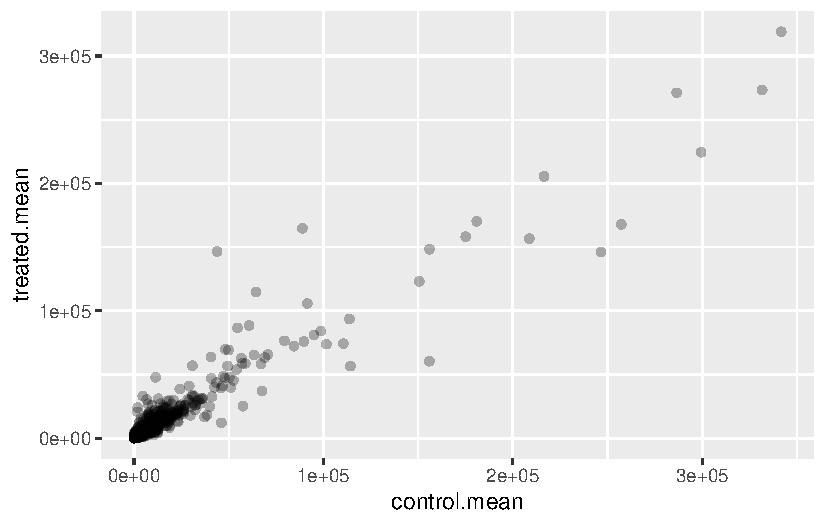
\includegraphics{Transcriptomics"_files/figure-pdf/unnamed-chunk-16-1.pdf}

\begin{Shaded}
\begin{Highlighting}[]
\FunctionTok{plot}\NormalTok{(meancounts)}
\end{Highlighting}
\end{Shaded}

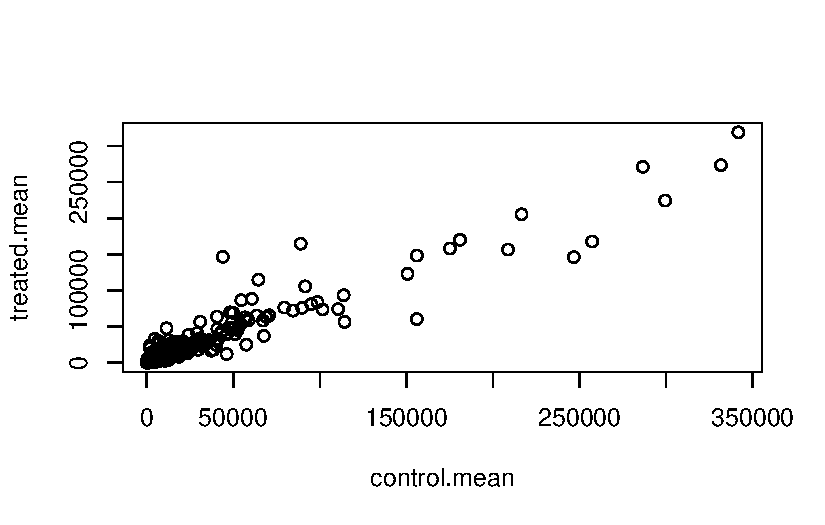
\includegraphics{Transcriptomics"_files/figure-pdf/unnamed-chunk-17-1.pdf}

\begin{quote}
Q5 (b).You could also use the ggplot2 package to make this figure
producing the plot below. What geom\_?() function would you use for this
plot?
\end{quote}

Geom\_point()

Whenever we see data that is so heavily skewed, like this, we often
transform it to log to see what is going on more easily.

\begin{quote}
Q6. Try plotting both axes on a log scale. What is the argument to
plot() that allows you to do this?
\end{quote}

log

\begin{Shaded}
\begin{Highlighting}[]
\FunctionTok{plot}\NormalTok{(}\FunctionTok{log}\NormalTok{(meancounts))}
\end{Highlighting}
\end{Shaded}

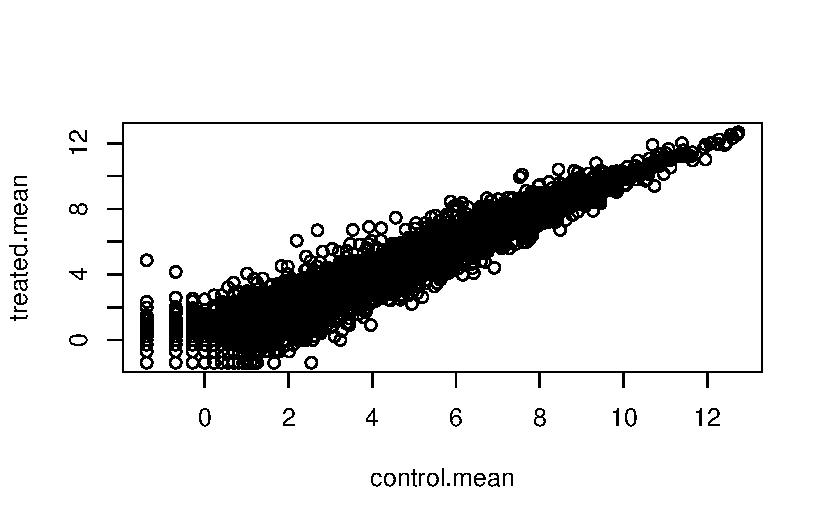
\includegraphics{Transcriptomics"_files/figure-pdf/unnamed-chunk-18-1.pdf}

We most often work in log2 units as this makes math easier. Let's have a
play to see this.

\begin{Shaded}
\begin{Highlighting}[]
\CommentTok{\# treated / control}
\FunctionTok{log2}\NormalTok{(}\DecValTok{20}\SpecialCharTok{/}\DecValTok{20}\NormalTok{)}
\end{Highlighting}
\end{Shaded}

\begin{verbatim}
[1] 0
\end{verbatim}

\begin{Shaded}
\begin{Highlighting}[]
\CommentTok{\#log2 of 1 is 0, therefore if there is a log2 change of 0 {-} there was no change }
\end{Highlighting}
\end{Shaded}

\begin{Shaded}
\begin{Highlighting}[]
\FunctionTok{log2}\NormalTok{(}\DecValTok{40}\SpecialCharTok{/}\DecValTok{20}\NormalTok{)}
\end{Highlighting}
\end{Shaded}

\begin{verbatim}
[1] 1
\end{verbatim}

\begin{Shaded}
\begin{Highlighting}[]
\CommentTok{\# going to have a log2 change of 1 }
\end{Highlighting}
\end{Shaded}

\begin{Shaded}
\begin{Highlighting}[]
\FunctionTok{log2}\NormalTok{(}\DecValTok{80}\SpecialCharTok{/}\DecValTok{20}\NormalTok{)}
\end{Highlighting}
\end{Shaded}

\begin{verbatim}
[1] 2
\end{verbatim}

\begin{Shaded}
\begin{Highlighting}[]
\CommentTok{\# going to have a log 2 change of 2 }
\end{Highlighting}
\end{Shaded}

\begin{Shaded}
\begin{Highlighting}[]
\CommentTok{\#treated/ control}
\FunctionTok{log2}\NormalTok{(}\DecValTok{20}\SpecialCharTok{/}\DecValTok{40}\NormalTok{)}
\end{Highlighting}
\end{Shaded}

\begin{verbatim}
[1] -1
\end{verbatim}

\begin{Shaded}
\begin{Highlighting}[]
\CommentTok{\# half as much treated as there is control, going into negatives}
\CommentTok{\# sign of the value tells which direction }
\CommentTok{\# 0 = on the line }
\CommentTok{\# positive = above the line }
\CommentTok{\# negative = below the line }
\end{Highlighting}
\end{Shaded}

Let's add ``log2 fold-change'' to our \texttt{meancounts} dataset.

\begin{Shaded}
\begin{Highlighting}[]
\NormalTok{meancounts}\SpecialCharTok{$}\NormalTok{log2fc }\OtherTok{\textless{}{-}} \FunctionTok{log2}\NormalTok{(meancounts}\SpecialCharTok{$}\NormalTok{treated.mean }\SpecialCharTok{/}\NormalTok{ meancounts}\SpecialCharTok{$}\NormalTok{control.mean)}
\end{Highlighting}
\end{Shaded}

There are a couple of ``weird'' results. Namely, the NaN (``not a
number'') and -Inf (negative infinity) results. The NaN is returned when
you divide by zero and try to take the log. The -Inf is returned when
you try to take the log of zero. It turns out that there are a lot of
genes with zero expression.

Let's filter out zero count genes - i.e.~remove the rows (genes) that
have a 0 value in either control or treated means.

How many genes are ``up'' regulated at the common log2 fold change
threshold of 2+?

\begin{Shaded}
\begin{Highlighting}[]
\NormalTok{up.inds }\OtherTok{\textless{}{-}}\NormalTok{ meancounts}\SpecialCharTok{$}\NormalTok{log2fc }\SpecialCharTok{\textgreater{}=} \DecValTok{2}
\FunctionTok{sum}\NormalTok{(up.inds, }\AttributeTok{na.rm =}\NormalTok{ T)}
\end{Highlighting}
\end{Shaded}

\begin{verbatim}
[1] 1910
\end{verbatim}

How many genes are ``down'' regulated at the threshold of -2?

\begin{Shaded}
\begin{Highlighting}[]
\NormalTok{down.inds }\OtherTok{\textless{}{-}}\NormalTok{ meancounts}\SpecialCharTok{$}\NormalTok{log2fc }\SpecialCharTok{\textgreater{}=} \SpecialCharTok{{-}}\DecValTok{2}
\FunctionTok{sum}\NormalTok{(down.inds, }\AttributeTok{na.rm =}\NormalTok{ T)}
\end{Highlighting}
\end{Shaded}

\begin{verbatim}
[1] 23046
\end{verbatim}

\begin{quote}
Q7. What is the purpose of the arr.ind argument in the which() function
call below? Why would we then take the first column of the output and
need to call the unique() function?
\end{quote}

The purpose of the \texttt{arr.ind} argument in the which() function is
being called is to return the row and column positions where it is
\texttt{TRUE}. This will tell which genes (rows) and samples (columns)
have 0 counts. The goal is to remove/ ignore any genes with 0 counts in
any of the samples so we can just focus on the row answer. The
\texttt{unique()} is being called to ensure that no row is being counted
twice if it has 0 entries in both samples.

\begin{Shaded}
\begin{Highlighting}[]
\NormalTok{zero.vals }\OtherTok{\textless{}{-}} \FunctionTok{which}\NormalTok{(meancounts[,}\DecValTok{1}\SpecialCharTok{:}\DecValTok{2}\NormalTok{]}\SpecialCharTok{==}\DecValTok{0}\NormalTok{, }\AttributeTok{arr.ind=}\ConstantTok{TRUE}\NormalTok{)}

\NormalTok{to.rm }\OtherTok{\textless{}{-}} \FunctionTok{unique}\NormalTok{(zero.vals[,}\DecValTok{1}\NormalTok{])}
\NormalTok{mycounts }\OtherTok{\textless{}{-}}\NormalTok{ meancounts[}\SpecialCharTok{{-}}\NormalTok{to.rm,]}
\FunctionTok{head}\NormalTok{(mycounts)}
\end{Highlighting}
\end{Shaded}

\begin{verbatim}
                control.mean treated.mean      log2fc
ENSG00000000003       900.75       658.00 -0.45303916
ENSG00000000419       520.50       546.00  0.06900279
ENSG00000000457       339.75       316.50 -0.10226805
ENSG00000000460        97.25        78.75 -0.30441833
ENSG00000000971      5219.00      6687.50  0.35769358
ENSG00000001036      2327.00      1785.75 -0.38194109
\end{verbatim}

\begin{quote}
Q8. Using the up.ind vector above can you determine how many up
regulated genes we have at the greater than 2 fc level?
\end{quote}

250

\begin{quote}
Q9. Using the down.ind vector above can you determine how many down
regulated genes we have at the greater than 2 fc level?
\end{quote}

367

\begin{Shaded}
\begin{Highlighting}[]
\NormalTok{up.ind }\OtherTok{\textless{}{-}}\NormalTok{ mycounts}\SpecialCharTok{$}\NormalTok{log2fc }\SpecialCharTok{\textgreater{}} \DecValTok{2}
\NormalTok{down.ind }\OtherTok{\textless{}{-}}\NormalTok{ mycounts}\SpecialCharTok{$}\NormalTok{log2fc }\SpecialCharTok{\textless{}}\NormalTok{ (}\SpecialCharTok{{-}}\DecValTok{2}\NormalTok{)}
\FunctionTok{sum}\NormalTok{(up.ind)}
\end{Highlighting}
\end{Shaded}

\begin{verbatim}
[1] 250
\end{verbatim}

\begin{Shaded}
\begin{Highlighting}[]
\FunctionTok{sum}\NormalTok{(down.ind)}
\end{Highlighting}
\end{Shaded}

\begin{verbatim}
[1] 367
\end{verbatim}

\begin{quote}
Q10. Do you trust these results? Why or why not?
\end{quote}

These results cannot be fully trusted as we did not filter out
significant from non-significant results. Fold-change can pear large
without statistical significance, and therefore affect the results.
Since we haven't looked at significance, the results can be misleading.

\section{Setting up for DESeq/ DESeq
Analysis}\label{setting-up-for-deseq-deseq-analysis}

To do this the right way, we need to consider statistical significance
of the differences - not just their magnitude.

\begin{Shaded}
\begin{Highlighting}[]
\CommentTok{\#/ message: false}
\FunctionTok{library}\NormalTok{(DESeq2)}
\end{Highlighting}
\end{Shaded}

To use this package, it wants \texttt{countData} and \texttt{colData} in
a specific format

\begin{Shaded}
\begin{Highlighting}[]
\NormalTok{dds }\OtherTok{\textless{}{-}} \FunctionTok{DESeqDataSetFromMatrix}\NormalTok{(}\AttributeTok{countData=}\NormalTok{counts, }
                              \AttributeTok{colData=}\NormalTok{metadata, }
                              \AttributeTok{design=}\SpecialCharTok{\textasciitilde{}}\NormalTok{dex)}
\end{Highlighting}
\end{Shaded}

\begin{verbatim}
converting counts to integer mode
\end{verbatim}

\begin{verbatim}
Warning in DESeqDataSet(se, design = design, ignoreRank): some variables in
design formula are characters, converting to factors
\end{verbatim}

\begin{Shaded}
\begin{Highlighting}[]
\NormalTok{dds}
\end{Highlighting}
\end{Shaded}

\begin{verbatim}
class: DESeqDataSet 
dim: 38694 8 
metadata(1): version
assays(1): counts
rownames(38694): ENSG00000000003 ENSG00000000005 ... ENSG00000283120
  ENSG00000283123
rowData names(0):
colnames(8): SRR1039508 SRR1039509 ... SRR1039520 SRR1039521
colData names(4): id dex celltype geo_id
\end{verbatim}

\begin{Shaded}
\begin{Highlighting}[]
\NormalTok{dds }\OtherTok{\textless{}{-}} \FunctionTok{DESeq}\NormalTok{(dds)}
\end{Highlighting}
\end{Shaded}

\begin{verbatim}
estimating size factors
\end{verbatim}

\begin{verbatim}
estimating dispersions
\end{verbatim}

\begin{verbatim}
gene-wise dispersion estimates
\end{verbatim}

\begin{verbatim}
mean-dispersion relationship
\end{verbatim}

\begin{verbatim}
final dispersion estimates
\end{verbatim}

\begin{verbatim}
fitting model and testing
\end{verbatim}

Extract my results

\begin{Shaded}
\begin{Highlighting}[]
\NormalTok{res }\OtherTok{\textless{}{-}} \FunctionTok{results}\NormalTok{(dds)}
\FunctionTok{head}\NormalTok{(res)}
\end{Highlighting}
\end{Shaded}

\begin{verbatim}
log2 fold change (MLE): dex treated vs control 
Wald test p-value: dex treated vs control 
DataFrame with 6 rows and 6 columns
                  baseMean log2FoldChange     lfcSE      stat    pvalue
                 <numeric>      <numeric> <numeric> <numeric> <numeric>
ENSG00000000003 747.194195     -0.3507030  0.168246 -2.084470 0.0371175
ENSG00000000005   0.000000             NA        NA        NA        NA
ENSG00000000419 520.134160      0.2061078  0.101059  2.039475 0.0414026
ENSG00000000457 322.664844      0.0245269  0.145145  0.168982 0.8658106
ENSG00000000460  87.682625     -0.1471420  0.257007 -0.572521 0.5669691
ENSG00000000938   0.319167     -1.7322890  3.493601 -0.495846 0.6200029
                     padj
                <numeric>
ENSG00000000003  0.163035
ENSG00000000005        NA
ENSG00000000419  0.176032
ENSG00000000457  0.961694
ENSG00000000460  0.815849
ENSG00000000938        NA
\end{verbatim}

\begin{quote}
padj = p value adjusted
\end{quote}

Plot of Fold Change vs.~P-Value (adjusted for multiple testing)

\begin{Shaded}
\begin{Highlighting}[]
\FunctionTok{plot}\NormalTok{(res}\SpecialCharTok{$}\NormalTok{log2FoldChange, res}\SpecialCharTok{$}\NormalTok{padj)}
\end{Highlighting}
\end{Shaded}

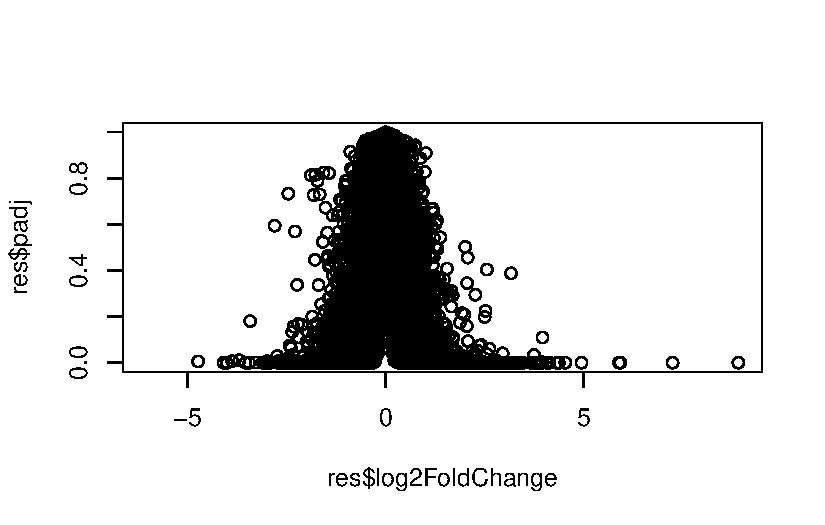
\includegraphics{Transcriptomics"_files/figure-pdf/unnamed-chunk-32-1.pdf}

\begin{quote}
fold change of 0 = no change, negative = downregulated, positive = up
regulated
\end{quote}

\begin{quote}
the higher the p-value = the less significant it is WE WANT SMALL
P-VALUES (downwards values)
\end{quote}

Take the log of the P-Value

\begin{Shaded}
\begin{Highlighting}[]
\FunctionTok{plot}\NormalTok{(res}\SpecialCharTok{$}\NormalTok{log2FoldChange, }\FunctionTok{log}\NormalTok{(res}\SpecialCharTok{$}\NormalTok{padj))}
\end{Highlighting}
\end{Shaded}

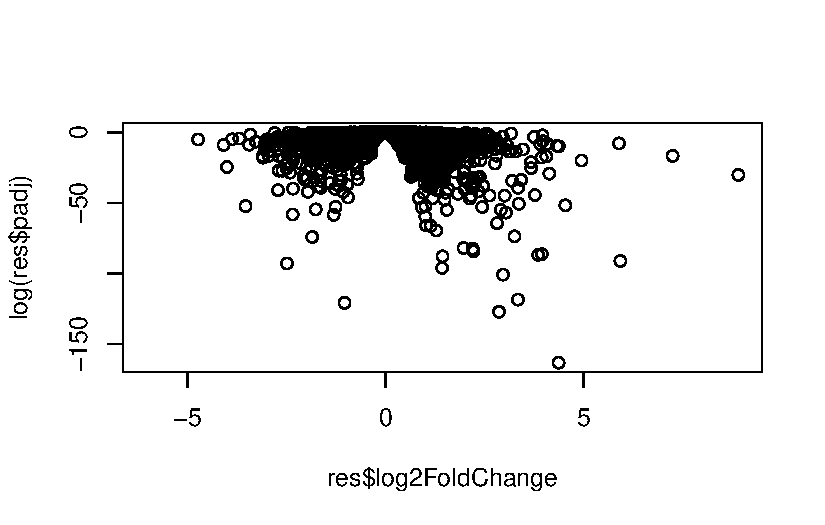
\includegraphics{Transcriptomics"_files/figure-pdf/unnamed-chunk-33-1.pdf}

\begin{quote}
In this plot, look down the axis.
\end{quote}

\begin{Shaded}
\begin{Highlighting}[]
\FunctionTok{log}\NormalTok{(}\FloatTok{0.01}\NormalTok{)}
\end{Highlighting}
\end{Shaded}

\begin{verbatim}
[1] -4.60517
\end{verbatim}

\begin{Shaded}
\begin{Highlighting}[]
\FunctionTok{log}\NormalTok{(}\FloatTok{0.00000001}\NormalTok{)}
\end{Highlighting}
\end{Shaded}

\begin{verbatim}
[1] -18.42068
\end{verbatim}

\begin{quote}
the smaller the p-value, the higher the negative number = greater
significance
\end{quote}

We can flip the y-axis by putting a minus sign on it

\begin{Shaded}
\begin{Highlighting}[]
\FunctionTok{plot}\NormalTok{(res}\SpecialCharTok{$}\NormalTok{log2FoldChange, }\SpecialCharTok{{-}}\FunctionTok{log}\NormalTok{(res}\SpecialCharTok{$}\NormalTok{padj), }
     \AttributeTok{xlab =} \StringTok{"Log2 Fold{-}Change"}\NormalTok{, }
     \AttributeTok{ylab =} \StringTok{"{-}log(P{-}value"}\NormalTok{)}
\end{Highlighting}
\end{Shaded}

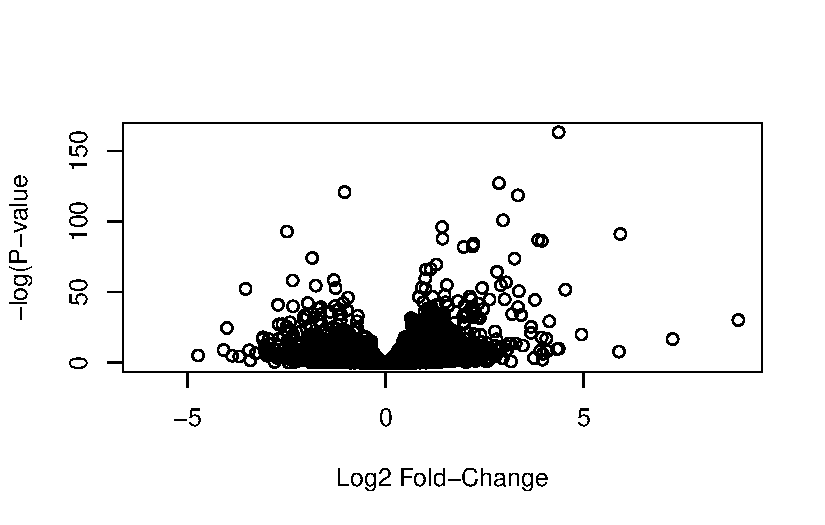
\includegraphics{Transcriptomics"_files/figure-pdf/unnamed-chunk-36-1.pdf}

\begin{quote}
standard volcano plot
\end{quote}

Let's save our work to date

\begin{Shaded}
\begin{Highlighting}[]
\FunctionTok{write.csv}\NormalTok{(res, }\AttributeTok{file =} \StringTok{"myresults.csv"}\NormalTok{)}
\end{Highlighting}
\end{Shaded}

To finish off, let's make a nicer volcano plot. Use ggplot. - Add the
log2 threshold lines of +2/-2 - Add P-value threshold lines at 0.05, -
Add color to highlight the subset of genes that meet both of the above
thresholds.

\begin{Shaded}
\begin{Highlighting}[]
\NormalTok{mycols }\OtherTok{\textless{}{-}} \FunctionTok{rep}\NormalTok{(}\StringTok{"gray"}\NormalTok{, }\FunctionTok{nrow}\NormalTok{(res))}
\NormalTok{mycols[res}\SpecialCharTok{$}\NormalTok{log2FoldChange }\SpecialCharTok{\textgreater{}=} \DecValTok{2}\NormalTok{] }\OtherTok{\textless{}{-}} \StringTok{"red"}
\NormalTok{mycols[res}\SpecialCharTok{$}\NormalTok{log2FoldChange }\SpecialCharTok{\textless{}=} \SpecialCharTok{{-}}\DecValTok{2}\NormalTok{] }\OtherTok{\textless{}{-}} \StringTok{"blue"}
\NormalTok{mycols[res}\SpecialCharTok{$}\NormalTok{padj }\SpecialCharTok{\textgreater{}} \FloatTok{0.05}\NormalTok{] }\OtherTok{\textless{}{-}} \StringTok{"gray"}
\end{Highlighting}
\end{Shaded}

\begin{Shaded}
\begin{Highlighting}[]
\FunctionTok{ggplot}\NormalTok{(res) }\SpecialCharTok{+}
  \FunctionTok{aes}\NormalTok{(log2FoldChange, }\SpecialCharTok{{-}}\FunctionTok{log}\NormalTok{(padj))}\SpecialCharTok{+}
  \FunctionTok{geom\_point}\NormalTok{(}\AttributeTok{col=}\NormalTok{mycols) }\SpecialCharTok{+}
  \FunctionTok{geom\_vline}\NormalTok{(}\AttributeTok{xintercept =} \FunctionTok{c}\NormalTok{(}\SpecialCharTok{{-}}\DecValTok{2}\NormalTok{,}\DecValTok{2}\NormalTok{), }\AttributeTok{col=}\StringTok{"red"}\NormalTok{) }\SpecialCharTok{+}
  \FunctionTok{geom\_hline}\NormalTok{(}\AttributeTok{yintercept =} \FloatTok{0.05}\NormalTok{, }\AttributeTok{col=}\StringTok{"blue"}\NormalTok{)}
\end{Highlighting}
\end{Shaded}

\begin{verbatim}
Warning: Removed 23549 rows containing missing values or values outside the scale range
(`geom_point()`).
\end{verbatim}

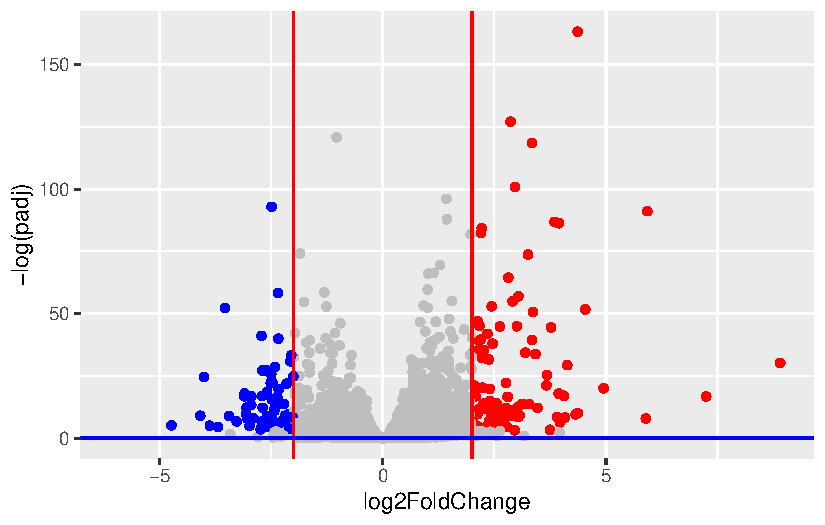
\includegraphics{Transcriptomics"_files/figure-pdf/unnamed-chunk-39-1.pdf}




\end{document}
